\documentclass{article}

\usepackage{graphicx}      % needed for including graphics e.g. EPS, PS
\usepackage{epstopdf}      % automatic conversion
\usepackage{grffile}       % allow fullstops in graphics file names
\usepackage[format=hang,singlelinecheck=0,font={sf,small},labelfont=bf]{caption, subfig}
                          % allow subfigures
\usepackage[noabbrev]{cleveref}      % reference object types automatically

\graphicspath{{figures/}}

\begin{document}

Here is some text and a figure

\begin{figure}

  \begin{minipage}[tbh]{\linewidth}
    \centering
    \captionsetup{justification=raggedright}
    \subfloat[text]{\includegraphics[width=0.3\textwidth]{logo.jpg}}\qquad
    \subfloat[text]{\label{fig:}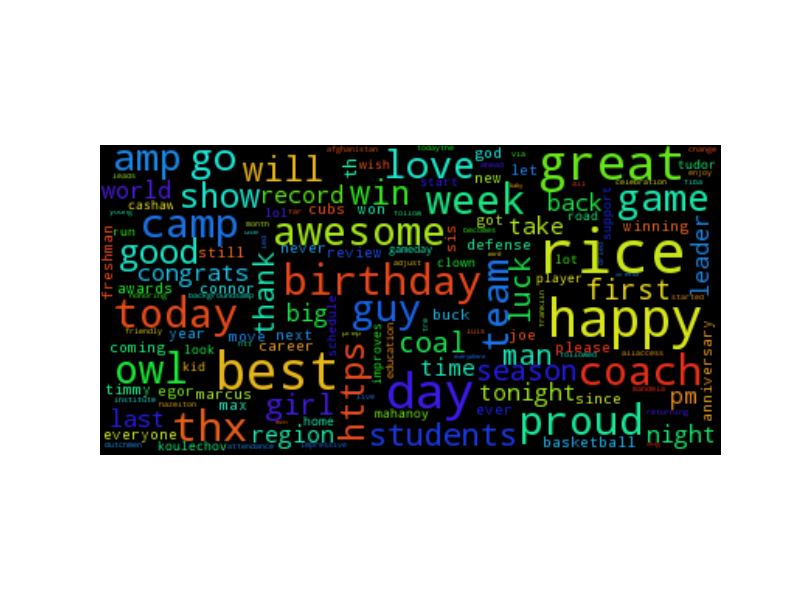
\includegraphics[width=0.3\textwidth]{wordcloud.png}}\qquad

%
 %   \subfloat[text]{\label{fig:1c}\includegraphics{file3.eps}}\qquad
  %  \subfloat[text]{\label{fig:1d}\includegraphics{file4.eps}}\qquad

  \end{minipage}

%  \caption{\subref{fig:1a} to \subref{fig:1b} are plotted against height, and \subref{fig:1c} to %\subref{fig:1d} against pressure}
  \label{fig:1}

\end{figure}

Now I'd like to refer to the figure \ref{fig:1d}. And use cref: \cref{fig:1d}

\end{document}